\section{Placa de expansión para el agente robótico}

Luego de haber probado todos los sistemas en conjunto se procedió a diseñar
una placa de expansión para el agente robótico Pololu 3Pi+ que permita
la conexión de todos los sistemas diseñados. Para permitir la conexión
 entre ambas placas se utilizaron conectores 
macho ubicados según los planos proporcionados por la 
empresa Pololu \cite{noauthor_pololu_nodate}.
Los pines utilizados para la comunicación o transmisión de potencia entre
ambas placas son los siguientes:

\begin{itemize}
    \item GND: Todos los pines etiquetados como GND en la placa de control
    del agente robótico son conectados con la tierra de la placa de expansión.
    \item VBAT: Este pin es utilizado para realizar la carga de las baterías
    NiMH presentes en el agente robótico.
    \item VSW: Este pin es utilizado para alimentar la placa de 
    control del agente robótico, al momento de que la batería NiMH 
    se encuentre descargada.

\end{itemize}

Debido a la alta cantidad de componentes que se encuentran en la placa de expansión
se decidió utilizar una placa de 4 capas, con el fin de facilitar el enrutamiento
de las señales de potencia y de comunicación entre los distintos componentes. 
La placa de expansión diseñada se muestra en la figura \ref{fig:expansion_board}.

\begin{figure}[H]
    \centering
    \begin{subfigure}{0.45\textwidth}
        \centering
        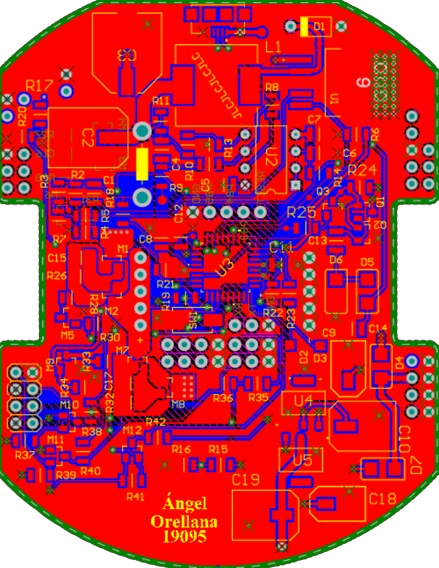
\includegraphics[scale=0.3]{imagenes/system_top.png}
        \caption{Capa superior}
    \end{subfigure}
    \begin{subfigure}{0.45\textwidth}
        \centering
        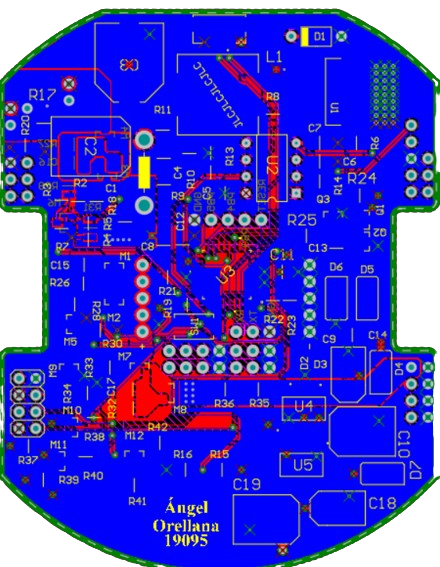
\includegraphics[scale=0.3]{imagenes/system_bottom.png}
        \caption{Capa inferior}
    \end{subfigure}
    \vfill
    \begin{subfigure}{0.45\textwidth}
        \centering
        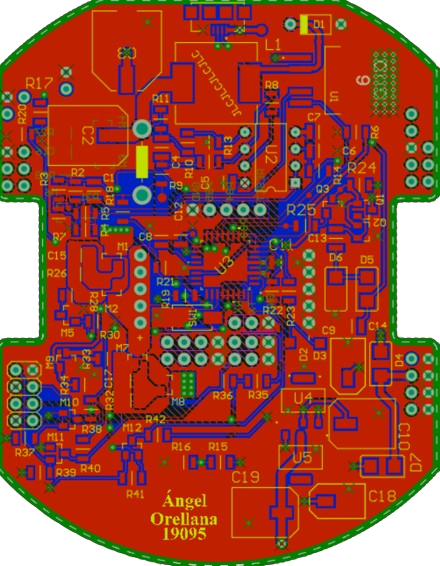
\includegraphics[scale=0.3]{imagenes/system_gnd.png}
        \caption{Plano de tierra de la placa de expansión} 
    \end{subfigure}
    \begin{subfigure}{0.45\textwidth}
        \centering
        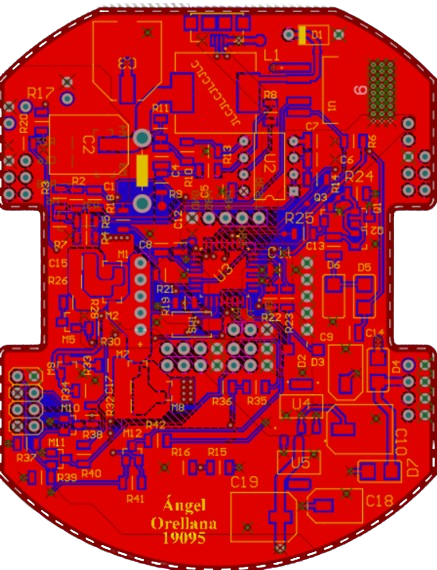
\includegraphics[scale=0.3]{imagenes/system_pwr.png}
        \caption{Plano de potencia de la placa de expansión}
    \end{subfigure}

    \caption{Placa de expansión para el agente robótico}
    \label{fig:expansion_board}
\end{figure}

Para comprobar que la placa de expansión diseñada se alinea correctamente
con la placa de control del agente robótico se realizó descargó el modelo
3D de la placa de control del agente robótico desde la página web de Pololu
\cite{noauthor_pololu_nodate}, y se realizó el ensamblaje de ambas placas
en el software Altium Designer, el resultado del ensamblaje se muestra en
la figura \ref{fig:expansion_board_assembly}.

\begin{figure}[H]
    \centering
    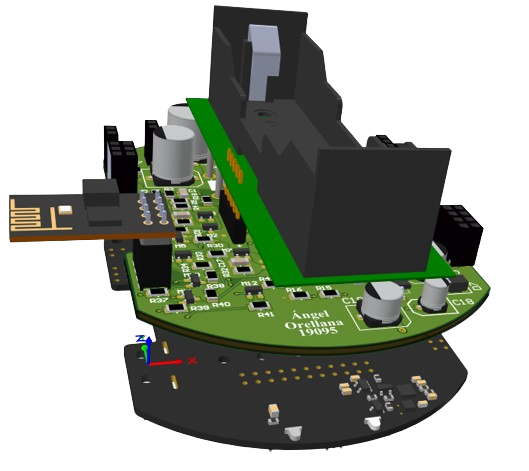
\includegraphics[scale=0.5]{imagenes/system_assembly.png}
    \caption{Ensamblaje de la placa de expansión con la placa de control del agente robótico}
    \label{fig:expansion_board_assembly}
\end{figure}

\subsection{Pruebas de la placa de expansión}

Para comprobar el correcto funcionamiento de la placa de expansión diseñada,
principalmente se realizaron pruebas de comunicación entre la placa de expansión
y la placa de control del agente robótico, y pruebas de alimentación de la placa
de control del agente robótico. Para comprobar que no existiera una interrupción
en la alimentación de la placa de control del agente robótico al momento de 
realizar el cambio de batería se utilizó el programa mostrado en el apéndice
\ref{sec:codigo_prueba_expansion}, el cual corresponde al proyecto de MPLAB
nombrado como Pololu\_on\_test.X, dentro de la carpeta nombrada como Charge\_system\_firmware.

En la figura \ref{fig:expansion_board_test} se muestra la placa de expansión
conectada a la placa de control del agente robótico.

\begin{figure}[H]
    \centering
    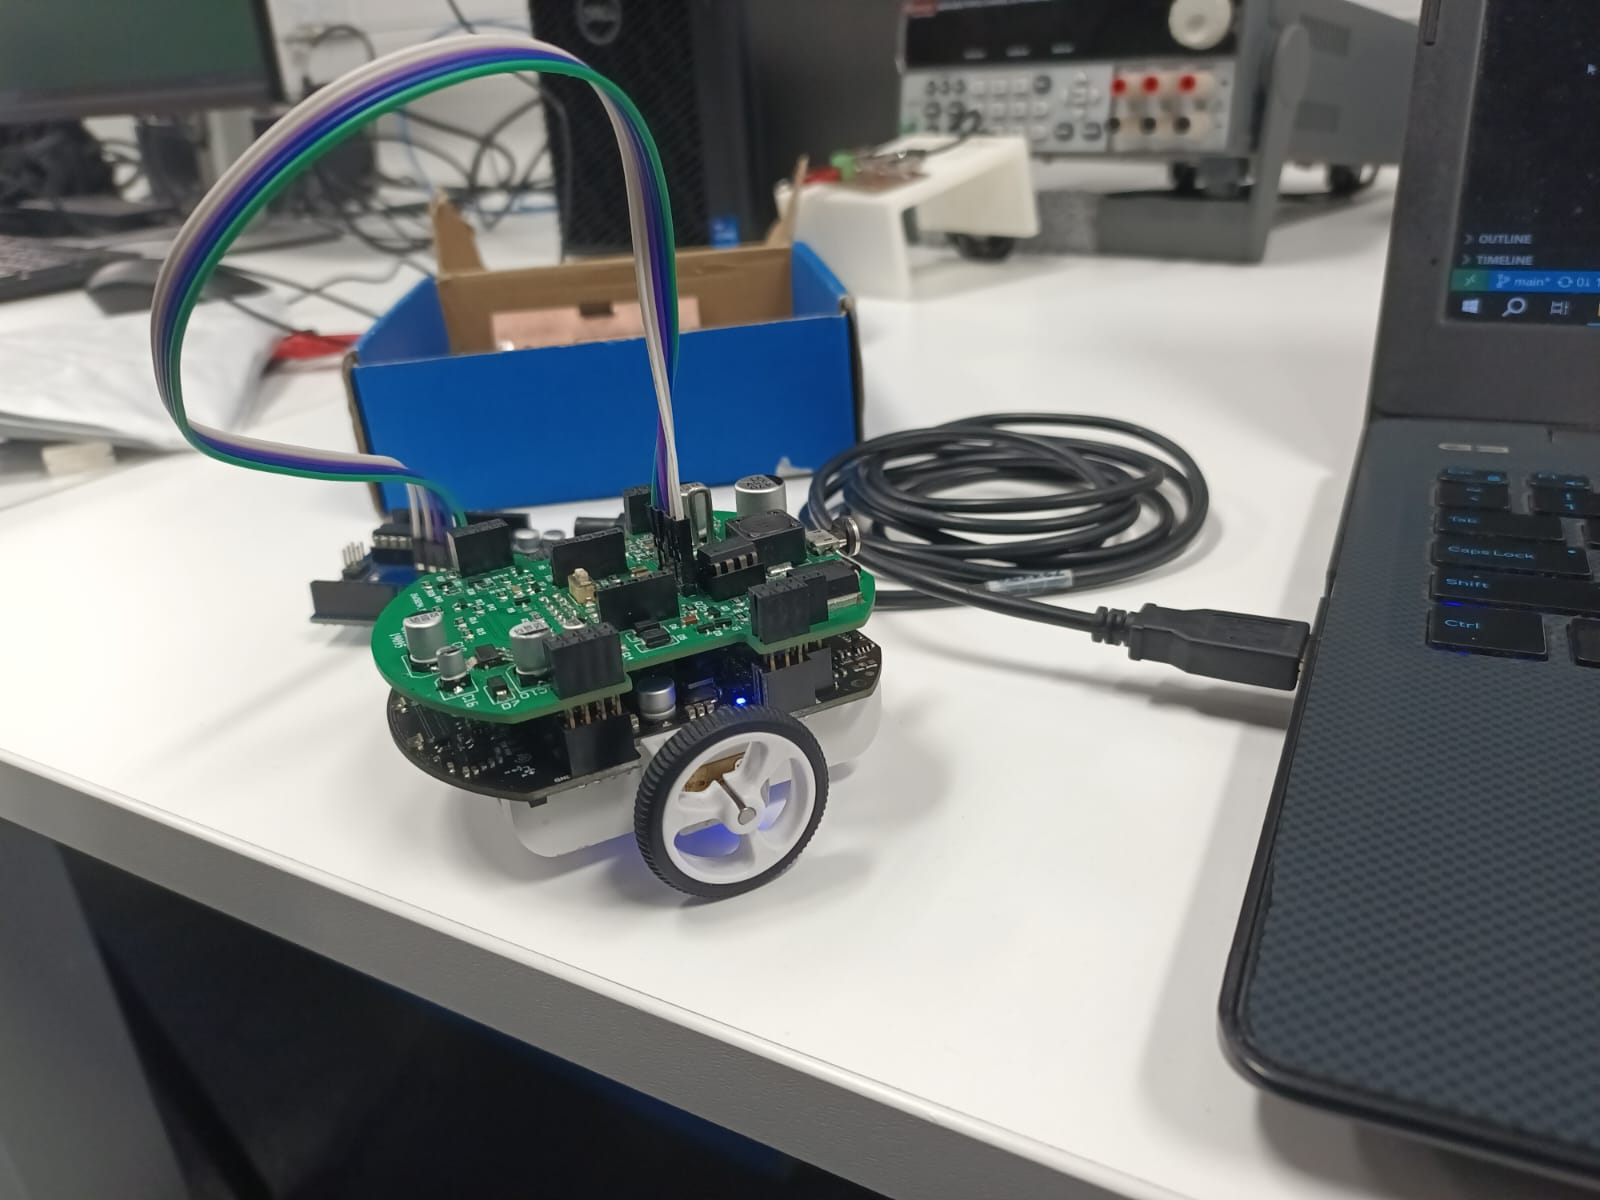
\includegraphics[scale=0.2]{imagenes/system_test.jpg}
    \caption{Prueba de la placa de expansión}
    \label{fig:expansion_board_test}
\end{figure}

El programa final de la placa de expansión se muestra en el apéndice \ref{sec:codigo_expansion},
el cual corresponde al proyecto de MPLAB nombrado como Pololu\_on.X, dentro de la carpeta

